%%=============================================================================
%% Methodologie
%%=============================================================================

\chapter{\IfLanguageName{dutch}{Methodologie}{Methodology}}%
\label{ch:methodologie}

%% TODO: In dit hoofstuk geef je een korte toelichting over hoe je te werk bent
%% gegaan. Verdeel je onderzoek in grote fasen, en licht in elke fase toe wat
%% de doelstelling was, welke deliverables daar uit gekomen zijn, en welke
%% onderzoeksmethoden je daarbij toegepast hebt. Verantwoord waarom je
%% op deze manier te werk gegaan bent.
%% 
%% Voorbeelden van zulke fasen zijn: literatuurstudie, opstellen van een
%% requirements-analyse, opstellen long-list (bij vergelijkende studie),
%% selectie van geschikte tools (bij vergelijkende studie, "short-list"),
%% opzetten testopstelling/PoC, uitvoeren testen en verzamelen
%% van resultaten, analyse van resultaten, ...
%%
%% !!!!! LET OP !!!!!
%%
%% Het is uitdrukkelijk NIET de bedoeling dat je het grootste deel van de corpus
%% van je bachelorproef in dit hoofstuk verwerkt! Dit hoofdstuk is eerder een
%% kort overzicht van je plan van aanpak.
%%
%% Maak voor elke fase (behalve het literatuuronderzoek) een NIEUW HOOFDSTUK aan
%% en geef het een gepaste titel.

Dit hoofdstuk bespreekt kort de fasen van het onderzoek. Per fase word kort besproken wat de doelstelling is en welke keuzes gemaakt werden. In figuur \ref{fig:flow-chart} wordt een overzicht getoond van de verschillende fasen en hoe deze elkaar opvolgen.

\paragraph{Literatuurstudie en modellen zoeken}
Deze fase bestaat uit het opzoeken van info omtrent diarization en welke bestaande modellen hier al voor zijn. Hieruit worden de modellen gekozen die het meeste potentieel lijken te hebben om tot een goed eindresultaat te komen en wordt gekeken wat de beste manier van aanpakken is.\\
Naast het zoeken naar modellen, wordt ook gezocht naar methoden om deze modellen te evalueren. Dit zorgt ervoor dat er een gegronde keuze kan gemaakt worden om verder te gaan met een specifiek model. Dit zorgt er in een latere fase ook voor dat er gekozen kan worden voor de beste parameters voor het model.

\paragraph{Modellen testen}
Tijdens deze fase wordt getest hoe bruikbaar de gevonden modellen effectief zijn en wat het beste model is om mee verder te gaan. Dit wordt gedaan door eerst te kijken naar het gemak om het model te installeren en lokaal werkend te krijgen. Hierna wordt een audiofragment gegeven aan de modellen en wordt gekeken naar de accuraatheid waarmee elk model de stemmen in dit fragment al kan onderscheiden. Uiteindelijk wordt er ook gekeken naar de mogelijkheid om het model verder te trainen om een beter resultaat te kunnen bekomen. Op basis van deze criteria wordt dan gekozen met welk model verder gegaan wordt in de volgende fasen.

\paragraph{Voorbereiden van de trainingsdata}
In deze fase wordt gezocht naar bruikbare Vlaamse audiofragmenten. Voornamelijk wordt gezocht naar Vlaamse televisieprogramma's en podcasts op \url{hetarchief.be} en YouTube. Op basis van de gevonden audio worden dan RTTM- en UEM-bestanden geschreven en afhankelijk van het gekozen model op de juiste manier opgeslagen. RTTM (Rich Transcription Time Marked) is een tekstgebaseerd bestandstype die bestaat uit tijdsmarkeringen die aangeven wanneer een woord of zin start en eindigt en die voornamelijk gebruikt wordt in spraak herkennende software \autocite{filext}. UEM (Un-partitioned Evaluation Map) bestanden worden gebruikt om aan te duiden welke delen van de audiobestanden gebruikt zijn om de RTTM-bestanden op te stellen \autocite{Ryant}.

\paragraph{Model trainen en finetunen}
Tijdens deze fase wordt het gekozen model getraind aan de hand van de data uit de vorige fase. Voor en na het trainen wordt het model geëvalueerd, aan de hand van methoden die in de eerste fase gevonden werden, om te kijken of het trainen het model accurater maakt dan het was voor het trainen. Hierna zullen de parameters van het model verder gefinetuned worden, waarna de accuraatheid opnieuw geëvalueerd wordt en eventueel meer finetuning plaatsvindt, tot een zo accuraat mogelijk model bekomen wordt.

\paragraph{Implementatie in de applicatie}
In deze laatste fase zal het model opgeslagen worden en geïmplementeerd worden in de broncode van de reeds bestaande applicatie. Er zal ook grondig getest worden of het model hierin het beoogde resultaat heeft.

\begin{figure}
	\centering
	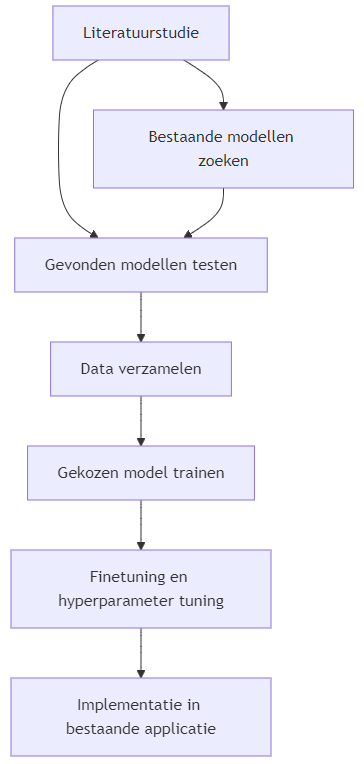
\includegraphics[scale=0.75]{./img/verloop.png}
	\caption[Voorstelling van de fasen van het onderzoek]{\label{fig:flow-chart}Voorstelling van de fasen van de bachelorproef en hun onderlinge volgorde}
\end{figure}